\documentclass[reprint, amsmath, amssymb, aps, prl]{revtex4-2}

\usepackage{graphicx}
\graphicspath{{./assets/figures/}}
\usepackage{dcolumn}
\usepackage{bm}
\usepackage{diagbox}
\usepackage[table]{xcolor}
\usepackage{empheq} % to use left braces for list of equations
\usepackage{hyperref}

\begin{document}

\preprint{APS/123-QED}

\title{Energy spectrum of diatomic molecules\\ in the Quantum Drude Oscillator model}
%\thanks{}

\author{Matthieu Sarkis}
\email{matthieu.sarkis@uni.lu}

\author{Loris di Cairano}%
\email{loris.dicairano@uni.lu}

\author{Alexandre Tkatchenko}%
\email{alexandre.tkatchenko@uni.lu}

\affiliation{
Department of Physics and Materials Science\\ University of Luxembourg, L-1511, Luxembourg City, Luxembourg.
}

%\collaboration{}%\noaffiliation

\date{\today}

\begin{abstract}
Abstract
%\begin{description}
%\item[Usage]
%Secondary publications and information retrieval purposes.
%\item[Structure]
%You may use the \texttt{description} environment to structure your abstract;
%use the optional argument of the \verb+\item+ command to give the category of each item.
%\end{description}
\end{abstract}

%\keywords{Suggested keywords}%Use showkeys class option if keyword
                              %display desired
\maketitle

%\tableofcontents

\section{Introduction}

    A Quantum Drude Oscillator (QDO) is a very simple atomistic model in which the properties of an atom are encompassed in a small number of parameters. The model consists in assimilating the atom to a point particle of mass $m$ and electric charge $-q$ attached to a fixed (infinite mass) center of charge $+q$ by a harmonic spring characterized by a frequency $\omega$. Molecules are then defined as a collections of QDOs interactig through Coulomb interactions.

    \begin{figure}[h!]
    \centering
        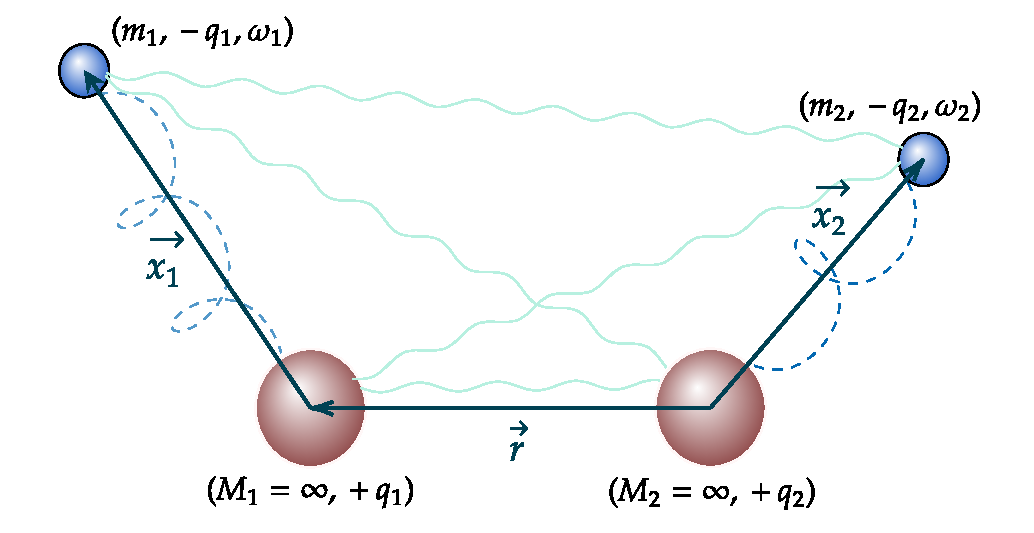
\includegraphics[scale=0.49]{QDOs}
        \caption{\label{fig:epsart} Pair of interacting QDOs.}
    \end{figure}

    This simple model has been extensively used in various contexts, for instance in order to tackle the electronic structure problem for isolated molecules, in particular long range interactions, as well as to study the impact of an ambient bath or of an external electric field on molecular properties \cite{Karimpour_2022}.

    Even though the harmonic oscillator nature of the atomic constituents in this model drastically simplify the complexity of problem, the all-body Coulomb interaction remains challenging. One possible way to proceed is to treat the Coulomb interaction by performing a multipolar expansion.

    By truncating the multipolar expansion up to Dipole-Dipole, one obtain a quadratic Hamiltonian, hence the quantum Hamiltonian can be analytically diagonalized. Though simple, this system was shown to capture long-range phenomena in large atomistic systems \cite{https://doi.org/10.48550/arxiv.2205.11549}.

    In the present work, we focus instead on small (diatomic) molecules in 1d, and treat in an \textit{analytical} way the Coulombic interactions up to Quadrupole-Quadrupole and Dipole-Octupole order, paving the way towards generalization for larger systems.

    \textit{GitHub repository}: The reader will find an open source code accompanying this paper following this \href{https://github.com/MatthieuSarkis/Quartic-Potential}{link}.

\section{Quartic Hamiltonian for diatomic molecules}

    \subsection{Multipolar expansion for the Coulomb potential}

        The Hamiltonian describing a system of $N$ QDOs in 3d is given by:
        \begin{equation}
        \label{eq:full_QDO_Hamiltonian}
            H=\sum_{i=1}^N\left[\frac{1}{2}m_i\dot{\vec x}_i^2 + \frac{1}{2}m_i\omega_i^2\vec x_i^2\right] +\sum_{i<j}V_\text{Coul}\left(\vec x_i, \vec x_j\right)\,,
        \end{equation}
        with the Coulomb interaction given by
        \begin{equation*}
            \frac{V_\text{Coul}\left(\vec x_1, \vec x_2\right)}{q_1q_2(4\pi\epsilon_0)^{-1}}=\frac{1}{r} - \frac{1}{|\vec r + \vec x_1|} - \frac{1}{|\vec r - \vec x_2|} + \frac{1}{|\vec r - \vec x_2 + \vec x_1|}
        \end{equation*}
        In the multipolar expansion, this can be expressed as:
        \begin{equation}
            V_\text{Coul}\left(\vec x_1, \vec x_2\right)= \sum_{n\geq 0} V_n\left(\vec x_1, \vec x_2\right)\,,
        \end{equation}
        with the following scaling behavior in terms of the distance between the centers:
        \begin{equation}
            V_n\left(\vec x_1, \vec x_2\right)\propto r^{-n+3}\,.
        \end{equation}
        The first terms in that multipolar expansion have the following interpretation:
        \begin{itemize}
            \item $n=0$ : Dipole-Dipole interaction (DD),
            \item $n=1$ : Dipole-Quadrupole interaction (DQ),
            \item $n=2$ : Quadrupole-Quadrupole and Dipole-Octupole interaction (QQ+DO).
        \end{itemize}
        Using the following identity for generic vectors $\vec r$ and $\vec \epsilon$:
        \begin{widetext}
        \begin{equation}
            \frac{1}{\left|\vec r - \vec\epsilon\,\right|} = \frac{1}{r}\left[1 + \frac{\vec\epsilon\cdot\hat r}{r} - \frac{\epsilon^2 - 3(\vec\epsilon\cdot\hat r)^2}{2r^2}+\frac{5(\vec\epsilon\cdot\hat r)^3-3\epsilon^2(\vec\epsilon\cdot\hat r)}{2r^3}+\frac{35(\vec\epsilon\cdot\hat r)^4-30\epsilon^2(\vec\epsilon\cdot\hat r)^2+3\epsilon^4}{8r^4}+\mathcal O\left(\frac{\epsilon^5}{r^5}\right)\right]
        \end{equation}
        \end{widetext}
        one can explicitely compute $V_0$, $V_1$ and $V_2$. Instead of writting out the expression of these potentials in full glory, let us now restrict ourselves to a system composed of $N=2$ QDOs.

    \subsection{Reduced particle system}

        Let us move to the center of mass frame, in which the dynamics reduces to that of an effective reduced particle:
        \begin{subequations}
        \begin{align}
            &\vec x:=\vec x_1 - \vec x_2\\
            &m_1\vec x_1 + m_2\vec x_2 = \vec 0\,.
        \end{align}
        \end{subequations}
        In terms of the reduced variable, a straightforward computation gives us:
        \begin{subequations}
        \begin{align}
            V_0(\vec x)=\,&-\frac{m_1m_2}{(m_1+m_2)^2}\cdot\frac{ x^2-3(\vec x\cdot\hat r)^2}{4\pi\epsilon_0r^3}\,,\\
            V_1(\vec x)=\,&\frac{3m_1m_2}{2(m_1+m_2)^2}\cdot\frac{(\vec x\cdot\hat r)\left(3x^2 - 5(\vec x\cdot\hat r)^2\right)}{4\pi\epsilon_0r^4}\,,\\
            V_2(\vec x)=\,&\frac{m_1m_2(2m_1^2+3m_1m_2+2m_2^2)}{4(m_1+m_2)^4}\times\\
            &\times\frac{3x^4 - 30(\vec x\cdot\hat r)^2 x^2+35(\vec x\cdot\hat r)^4}{4\pi\epsilon_0r^5}\nonumber\,.
        \end{align}
        \end{subequations}
        Let us now assume that the system is effectively one-dimensional, aligned along the direction on which the centers of the two QDOs are sitting. One obtain the following one-dimensional potentials for an effective particle of mass $m_1m_2 / (m_1+m_2)$:
        \begin{subequations}
        \begin{align}
            V_0(x)&=\frac{2m_1m_2}{(m_1+m_2)^2}\cdot\frac{2 x^2}{4\pi\epsilon_0r^3}\,,\\
            %V_1(x)&=-\frac{3m_1m_2}{(m_1+m_2)^2}\cdot\frac{\text{sgn}(\vec x\cdot\hat r)|x|x^2}{4\pi\epsilon_0r^4}=\mathbin{\textcolor{teal}{-\frac{3m_1m_2}{(m_1+m_2)^2}\cdot\frac{x^3}{4\pi\epsilon_0r^4}}}\,,\\
            V_1(x)&=-\frac{3m_1m_2}{(m_1+m_2)^2}\cdot\frac{x^3}{4\pi\epsilon_0r^4}\,,\\
            V_2(x)&=\frac{2m_1m_2(2m_1^2+3m_1m_2+2m_2^2)}{(m_1+m_2)^4}\cdot\frac{x^4}{4\pi\epsilon_0r^5}\,.
        \end{align}
        \end{subequations}
        Including the contribution of the harmonic potentials present in (\ref{eq:full_QDO_Hamiltonian}) and coupling the system to an external electric field, one finally obtain the following total one-dimensional potential:
        \begin{equation}
        \label{eq:quartic_potential}
            V(x) = \alpha x + \beta x^2 + \gamma x^3 + \delta x^4 \,,
        \end{equation}
        with the following expression of the coupling constants:
        \begin{subequations}
        \label{eq:coupling_constants}
        \begin{align}
            \alpha &= -\frac{m_1 q_2 + m_2 q_1}{m_1+m_2}\cdot \mathcal E\\
            \beta &= \frac{m_1m_2}{(m_1+m_2)^2}\cdot\frac{2q_1 q_2}{4\pi\epsilon_0r^3} + \frac{1}{2}\cdot\frac{m_1m_2}{m_1+m_2}\cdot\frac{m_1\omega_2^2+m_2\omega_1^2}{m_1+m_2}\\
            \gamma&=-\frac{m_1m_2}{(m_1+m_2)^2}\cdot\frac{3 q_1 q_2}{4\pi\epsilon_0r^4}\,,\\
            \delta&=\frac{2m_1m_2(2m_1^2+3m_1m_2+2m_2^2)}{(m_1+m_2)^4}\cdot\frac{q_1 q_2}{4\pi\epsilon_0r^5}\,.
        \end{align}
        \end{subequations}

\section{Analytic solution of the Schr\"odinger equation}

    In what follows, we define $k^2:=\frac{m_1+m_2}{m_1 m_2}\frac{\hbar^2}{2}$.
    Let us consider the time-independent Schr\"odinger equation
    \begin{equation}
        \left[\frac{\text{d}^2}{\text{d}x^2} + \frac{\epsilon - V(x)}{k^2}\right]\psi(x) = 0\,,
    \end{equation}
    where the potential $V$ is provided by (\ref{eq:quartic_potential}) and (\ref{eq:coupling_constants}).

    Following \cite{Lay_1998}, we solve the problem separately on the positive and negative real axis, and impose that the two solutions (positive and negative) $\psi_\pm$ and their first derivative match at the origin. For brievety reasons, we treat explicitely the case of the positive solution, the negative case being treated by perfoming the transformation $(x, \alpha, \beta, \gamma, \delta)\rightarrow (-x, -\alpha, \beta, -\gamma, \delta)$.

    Performing the following change of variable:
    \begin{equation}
        \psi_+(x)=\exp\left[\frac{\gamma^2-4\beta\delta}{8k\delta^{3/2}}\,x-\frac{\gamma}{4k\delta^{1/2}}\,x^2-\frac{\delta^{1/2}}{3k}\,x^3\right]\phi_+(x)
    \end{equation}
    we obtain:
    \begin{widetext}
    \begin{equation}
    \begin{split}
        &\frac{\text{d}^2\phi_+}{\text{d}x^2}(x)+\left[\frac{\gamma^2-4\beta\delta}{4k\delta^{3/2}}-\frac{\gamma}{k\delta^{1/2}}\,x-\frac{2\delta^{1/2}}{k}\,x^2\right]\frac{\text{d}\phi_+}{\text{d}x}(x)\\
        &+\left[\frac{16 \delta ^2 \left(\beta ^2+4 \delta  \epsilon \right)-8 \beta  \gamma ^2 \delta +\gamma ^4-32 \gamma  \delta ^{5/2} k}{64 \delta ^3 k^2}-\frac{8 \alpha  \delta ^2-4 \beta  \gamma  \delta +\gamma ^3+16 \delta ^{5/2} k}{8 \delta ^2 k^2}\,x\right]\phi_+(x)=0\,,
    \end{split}
    \end{equation}
    \end{widetext}
    which is known as the so-called \textit{tri-confluent Heun equation}.
    We further perform the following change of variable, the reason why to become clear soon:
    \begin{equation}
    \label{eq:change_variable}
        \phi_+(x)=(1+x)^{\frac{4 \beta  \gamma  \delta -\gamma ^3-8 \delta ^2 \left(\alpha +2k \delta^{1/2} \right)}{16k \delta ^{5/2}}}f_+(x)\,,
    \end{equation}
    as well as map the positive real axis to the segment $[0,1]$ through the change of argument
    \begin{equation}
        z=\frac{x}{x+1}\,,
    \end{equation}
    and look for a solution of the obtained ODE in terms of a series expansion at zero of the form:
    \begin{equation}
        f_+(z)=\sum_{n\geq 0}c^+_nz^n\,.
    \end{equation}
    Plugging the ansatz into the differential equation, we obtain the following recurrence relation between the coefficients:
    \begin{widetext}
    \begin{equation}
    \begin{split}
        &(n+1)(n+2) c^+_{n+2}+(n+1)(A -4n)c^+_{n+1} +[6(n-1) n+B n+E]c^+_n \\
        &+[C (n-1)+F-4(n-2) (n-1)]c^+_{n-1} + [(n-3) (n-2)+D (n-2)+G]c^+_{n-2}=0\ \ \ (n\geq 2)
    \end{split}
    \end{equation}
    \end{widetext}
    where the various coefficients are listed in full details in appendix. The change of variable (\ref{eq:change_variable}) is chosen precisely such that the order of the above difference equation is as small as possible. The coefficients $c^+_0$ and $c^+_1$ are to be fixed through boundary conditions, and the coeffients $c^+_2$ and $c^+_3$ are in turn fixed by the following relations
    \begin{equation}
    \begin{split}
        c^+_2&=-Ec^+_0-Ac^+_1\,,\\
        c^+_3&=-\frac{ F c^+_0+(B+E)c^+_1 +2 (A-4)c^+_2 }{6}\,.
    \end{split}
    \end{equation}
    Let us similarly denote by $c^-_n$ the coefficients in the series expansion corresponding to the solution on the negative real axis. It has been shown in \cite{Lay_1998} and \cite{doi:10.1063/1.531962} that the smooth matching of the two solutions at the origin can be achieved by imposing the so-called \textit{dominant solution} to the above defined difference equations vanishes. The conditions
    \begin{equation}
        \psi_+(0) = \psi_-(0)\ \ \ \text{and}\ \ \ \frac{\text{d}\psi_+}{\text{d}x}(0) = \frac{\text{d}\psi_-}{\text{d}x}(0)
    \end{equation}
    lead to constraints on the initial conditions for the difference equations, namely that $c^+_0 = c^-_0$ and:
    \begin{equation}
    \label{eq:initial_constraint}
    \begin{split}
        &c^+_1-c^+_0 \left[1+\frac{8 \delta ^2 (\alpha +\beta )-2 \gamma  \delta  (\gamma+2 \beta )+\gamma ^3}{16 \delta ^{5/2} k}\right]\\
        & = -c^-_1+c^-_0 \left[1-\frac{8 \delta ^2 (\alpha -\beta )+2 \gamma  \delta  (\gamma -2 \beta )+\gamma ^3}{16 \delta ^{5/2} k}\right]
    \end{split}
    \end{equation}
    The two sides of relation (\ref{eq:initial_constraint}) are therefore equal to some quantity $s$, which parameterizes the solution. Now, the vanishing of the dominant solution can be achieved by imposing that the series coefficients $c^+_n(\epsilon, s)$ and $c^-_n(\epsilon, s)$ are identically $0$ asymptotically in $n$. This provides a pair of algebraic equations in the energy variable $\epsilon$ and the \textit{shift} variable $s$.

    Let us make a few remarks at this stage. Imposing the vanishing of $c^\pm_n$ asymptotically in $n$ means that practically one should fix a large value of $n$, denote it $N$, and impose that the polynomials $c^\pm_N$ vanish. One observes that $c^-_N$ is a linear function of $s$. One can therefore solve explicitely for the shift variable in terms of the energy $\epsilon$. Plugging back into the other constraint, one obtains a rational function of the form:
    \begin{equation}
        c^+_N(\epsilon, s(\epsilon)) = \frac{P_N(\epsilon)}{Q_N(\epsilon)}
    \end{equation}
    where $P_n$ and $Q_N$ are polynomial functions of $\epsilon$, whose degree $d_N$ is an non-decreasing function of $N$. The $N$ zeros $\left\{\epsilon_i\right\}_{i=1}^N$ correspond then to first $N$ energy levels of the system, provided they are not complex and that $Q_N$ does not admit a zero of the same order.



\section{Results}

    \begin{table}[h!]
    \caption{\label{tab:Ar-Ar} Energy spectrum (in Ha) of the Ar-Ar system}
    \begin{ruledtabular}
    \begin{tabular}{c|ccc}
        \diagbox[height=1.8\line]{$r$ (a.u.)}{spectrum}& $\epsilon_0$ & $\epsilon_1$ & $\epsilon_2$ \\
        \hline
        0.5 & 9.247342 & 32.416619 & 62.971511 \\
        1.0 & 2.981229 & 10.350087 & 20.248422 \\
        1.5 & 1.563464 & 5.442288 & 10.069702 \\
        2.0 & 1.023301 & 3.394336 & 6.337199 \\
        2.5 & 0.748161 & 2.413177 & 4.876881 \\
        3.0 & 0.590991 & 1.960271 & 4.289340 \\  
    \end{tabular}
    \end{ruledtabular}
    \end{table}
    
    \begin{table}[h!]
    \caption{\label{tab:Cs-Cs} Energy spectrum (in Ha) of the Cs-Cs system}
    \begin{ruledtabular}
    \begin{tabular}{c|ccc}
        \diagbox[height=1.8\line]{$r$ (a.u.)}{spectrum}& $\epsilon_0$ & $\epsilon_1$ & $\epsilon_2$ \\
        \hline
        0.5 & 4.076335 & 14.287104 & 27.755741 \\
        1.0 & 1.307214 & 4.543529 & 8.897871 \\
        1.5 & 0.673427 & 2.362932 & 4.396492 \\
        2.0 & 0.426306 & 1.441411 & 2.686432 \\
        2.5 & 0.296956 & 0.971662 & 1.957474 \\
        3.0 & 0.217699 & 0.719613 & 1.585340 \\    
    \end{tabular}
    \end{ruledtabular}
    \end{table}
    
    \begin{table}[h!]
    \caption{\label{tab:H-H} Energy spectrum (in Ha) of the H-H system}
    \begin{ruledtabular}
    \begin{tabular}{c|ccc}
        \diagbox[height=1.8\line]{$r$ (a.u.)}{spectrum}& $\epsilon_0$ & $\epsilon_1$ & $\epsilon_2$ \\
        \hline
        0.5 & 3.757546 & 13.234211 & 25.693826 \\
        1.0 & 1.213930 & 4.243743 & 8.293979 \\
        1.5 & 0.649664 & 2.239448 & 4.116225 \\
        2.0 & 0.436524 & 1.423565 & 2.744604 \\
        2.5 & 0.330635 & 1.081656 & 2.284054 \\
        3.0 & 0.279296 & 0.965099 & 2.204208 \\      
    \end{tabular}
    \end{ruledtabular}
    \end{table}
    
    \begin{table}[h!]
    \caption{\label{tab:He-He} Energy spectrum (in Ha) of the He-He system}
    \begin{ruledtabular}
    \begin{tabular}{c|ccc}
        \diagbox[height=1.8\line]{$r$ (a.u.)}{spectrum}& $\epsilon_0$ & $\epsilon_1$ & $\epsilon_2$ \\
        \hline
        0.5 & 4.838555 & 16.998352 & 32.990230 \\
        1.0 & 1.609674 & 5.563162 & 10.796479 \\
        1.5 & 0.928052 & 3.096340 & 5.617631 \\
        2.0 & 0.690066 & 2.190579 & 4.209331 \\
        2.5 & 0.597424 & 1.987363 & 4.173586 \\
        3.0 & 0.607965 & 2.159394 & 4.851867 \\       
    \end{tabular}
    \end{ruledtabular}
    \end{table}
    
    \begin{table}[h!]
    \caption{\label{tab:K-K} Energy spectrum (in Ha) of the K-K system}
    \begin{ruledtabular}
    \begin{tabular}{c|ccc}
        \diagbox[height=1.8\line]{$r$ (a.u.)}{spectrum}& $\epsilon_0$ & $\epsilon_1$ & $\epsilon_2$ \\
        \hline
        0.5 & 3.900846 & 13.629450 & 26.449767 \\
        1.0 & 1.254074 & 4.338725 & 8.463017 \\
        1.5 & 0.646062 & 2.260433 & 4.233126 \\
        2.0 & 0.409452 & 1.389547 & 2.556108 \\
        2.5 & 0.286775 & 0.935829 & 1.841376 \\
        3.0 & 0.211508 & 0.689674 & 1.476942 \\         
    \end{tabular}
    \end{ruledtabular}
    \end{table}
    
    \begin{table}[h!]
    \caption{\label{tab:Kr-Kr} Energy spectrum (in Ha) of the Kr-Kr system}
    \begin{ruledtabular}
    \begin{tabular}{c|ccc}
        \diagbox[height=1.8\line]{$r$ (a.u.)}{spectrum}& $\epsilon_0$ & $\epsilon_1$ & $\epsilon_2$ \\
        \hline
        0.5 & 9.936548 & 34.839598 & 67.682787 \\
        1.0 & 3.196890 & 11.107797 & 21.743625 \\
        1.5 & 1.666467 & 5.817323 & 10.779216 \\
        2.0 & 1.078692 & 3.598874 & 6.723190 \\
        2.5 & 0.776461 & 2.514230 & 5.085759 \\
        3.0 & 0.599348 & 1.984794 & 4.360291 \\           
    \end{tabular}
    \end{ruledtabular}
    \end{table}
    
    \begin{table}[h!]
    \caption{\label{tab:Li-Li} Energy spectrum (in Ha) of the Li-Li system}
    \begin{ruledtabular}
    \begin{tabular}{c|ccc}
        \diagbox[height=1.8\line]{$r$ (a.u.)}{spectrum}& $\epsilon_0$ & $\epsilon_1$ & $\epsilon_2$ \\
        \hline
        0.5 & 2.989579 & 10.393189 & 20.094511 \\
        1.0 & 0.965106 & 3.317199 & 6.411919 \\
        1.5 & 0.498061 & 1.728672 & 3.276409 \\
        2.0 & 0.316132 & 1.076633 & 1.951989 \\
        2.5 & 0.223280 & 0.727240 & 1.384589 \\
        3.0 & 0.166518 & 0.533844 & 1.098635 \\              
    \end{tabular}
    \end{ruledtabular}
    \end{table}
    
    \begin{table}[h!]
    \caption{\label{tab:Ne-Ne} Energy spectrum (in Ha) of the Ne-Ne system}
    \begin{ruledtabular}
    \begin{tabular}{c|ccc}
        \diagbox[height=1.8\line]{$r$ (a.u.)}{spectrum}& $\epsilon_0$ & $\epsilon_1$ & $\epsilon_2$ \\
        \hline
        0.5 & 8.067324 & 28.257747 & 54.866835 \\
        1.0 & 2.648128 & 9.141505 & 17.802546 \\
        1.5 & 1.463214 & 4.975572 & 9.086247 \\
        2.0 & 1.037985 & 3.321372 & 6.216936 \\
        2.5 & 0.839105 & 2.707087 & 5.494303 \\
        3.0 & 0.769833 & 2.636825 & 5.742950 \\             
    \end{tabular}
    \end{ruledtabular}
    \end{table}
    
    \begin{table}[h!]
    \caption{\label{tab:Rb-Rb} Energy spectrum (in Ha) of the Rb-Rb system}
    \begin{ruledtabular}
    \begin{tabular}{c|ccc}
        \diagbox[height=1.8\line]{$r$ (a.u.)}{spectrum}& $\epsilon_0$ & $\epsilon_1$ & $\epsilon_2$ \\
        \hline
        0.5 & 4.031874 & 14.113400 & 27.409612 \\
        1.0 & 1.294297 & 4.489885 & 8.780383 \\
        1.5 & 0.666759 & 2.337266 & 4.359340 \\
        2.0 & 0.422361 & 1.430245 & 2.650383 \\
        2.5 & 0.294937 & 0.963709 & 1.922279 \\
        3.0 & 0.216807 & 0.712417 & 1.550805 \\                
    \end{tabular}
    \end{ruledtabular}
    \end{table}
    
    \begin{table}[h!]
    \caption{\label{tab:Xe-Xe} Energy spectrum (in Ha) of the Xe-Xe system}
    \begin{ruledtabular}
    \begin{tabular}{c|ccc}
        \diagbox[height=1.8\line]{$r$ (a.u.)}{spectrum}& $\epsilon_0$ & $\epsilon_1$ & $\epsilon_2$ \\
        \hline
        0.5 & 10.472412 & 36.762340 & 71.427248 \\
        1.0 & 3.360994 & 11.705550 & 22.941485 \\
        1.5 & 1.743863 & 6.103626 & 11.305873 \\
        2.0 & 1.117696 & 3.742926 & 7.034869 \\
        2.5 & 0.792188 & 2.580753 & 5.270133 \\
        3.0 & 0.598300 & 1.992258 & 4.438638 \\                 
    \end{tabular}
    \end{ruledtabular}
    \end{table}














    \begin{figure}[h!]
        \centering
            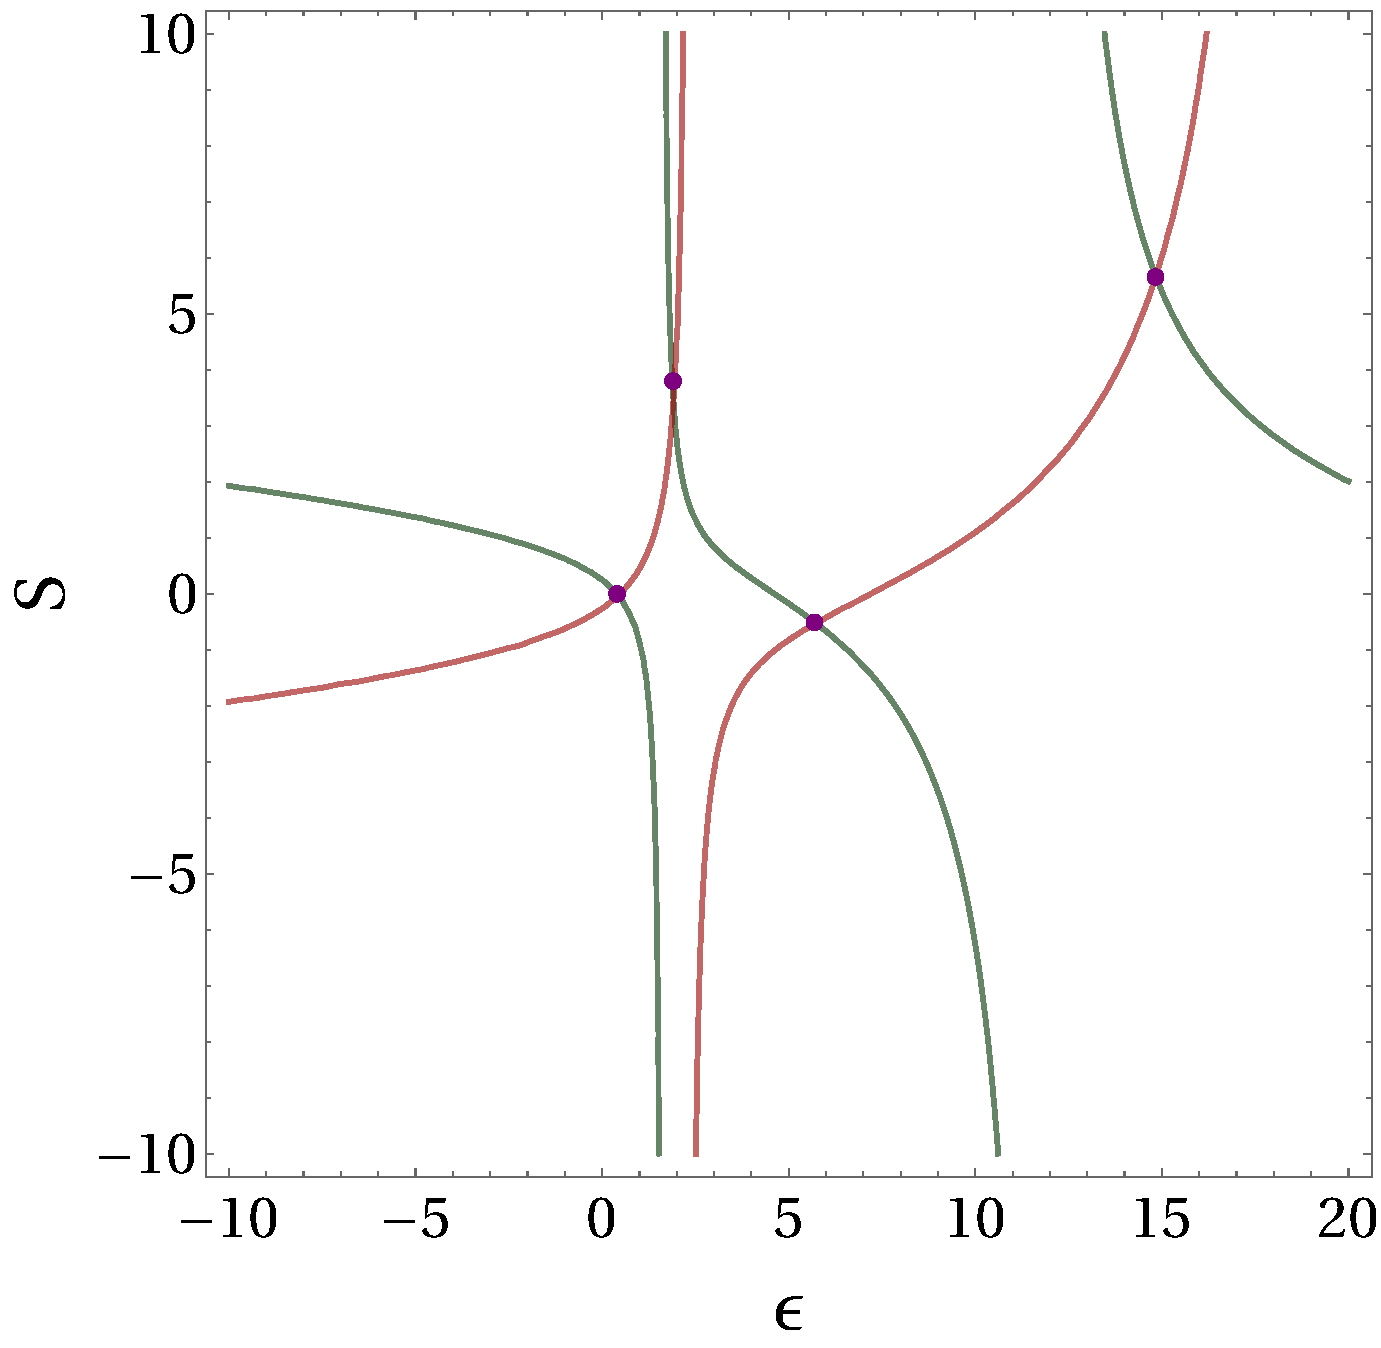
\includegraphics[scale=0.33]{plus_minus_coefs}
            \caption{\label{fig:coefs} Intersection loci of the three surfaces $z=c^+_{20}(\epsilon, s)$ and $z=c^-_{20}(\epsilon, s)$ and $z=0$. The purple dots correspond to the first excited states of the H-H system for $r=4$ and $\mathcal E=0$.}
    \end{figure}


%\begin{acknowledgments}
%We wish to acknowledge ...
%\end{acknowledgments}

\newpage

\appendix

\section{Atomic data}

    We collect here the QDO parameters obtained in \cite{PhysRevB.87.144103}.

    \begin{table}[h!]
    \caption{\label{tab:atomic_data} Parameters for QDOs (in a.u.)}
    \begin{ruledtabular}
    \begin{tabular}{c|ccc}
        & $\omega$ & $m$ & $q$ \\
        \hline
        H  & 0.4273 & 0.6099 & 0.7080 \\
        Li & 0.0687 & 1.2545 & 0.9848 \\
        K  & 0.0630 & 0.8101 & 0.9670 \\
        Rb & 0.0603 & 0.7343 & 0.9274 \\
        Cs & 0.0531 & 0.6939 & 0.8950 \\
        He & 1.0187 & 0.5083 & 0.8532 \\
        Ne & 1.2965 & 0.3491 & 1.2494 \\
        Ar & 0.7272 & 0.3020 & 1.3314 \\
        Kr & 0.6359 & 0.2796 & 1.3741 \\
        Xe & 0.5152 & 0.2541 & 1.3570
    \end{tabular}
    \end{ruledtabular}
    \end{table}

\section{Details on the derivation}

    \begin{widetext}
    \begin{equation*}
    \begin{split}
        A&=-\frac{8 \delta ^2 (\alpha +\beta )-2 \gamma  \delta  (2 \beta +\gamma )+\gamma ^3+32 \delta ^{5/2} k}{8 \delta ^{5/2} k}\\
        B&= \frac{8 \delta ^2 (3 \alpha +2 \beta -\gamma )-4 \gamma  \delta  (3 \beta +\gamma )+3 \gamma ^3+96 \delta ^{5/2} k}{8 \delta ^{5/2} k}\\
        C&= -\frac{8 \delta ^2 (3 \alpha +\beta -\gamma )-2 \gamma  \delta  (6 \beta +\gamma )+3 \gamma ^3+16 \delta ^3+96 \delta ^{5/2} k}{8 \delta ^{5/2} k}\\
        D&= \frac{-4 \beta  \gamma  \delta +\gamma ^3+8 \delta ^2 \left(\alpha +4 \sqrt{\delta } k\right)}{8 \delta ^{5/2} k}\\
        E&= \frac{4 \gamma ^2 \delta ^2 \left(\gamma  (4 \alpha +\gamma )+4 \beta ^2+8 \beta  \gamma \right)-32 \gamma  \delta ^3 (\alpha +\beta ) (2 \beta +\gamma )+64 \delta ^4 (\alpha +\beta )^2-4 \gamma ^4 \delta  (2 \beta +\gamma )}{256 \delta ^5 k^2}\\
       &\ \ \ \ \ \  +\frac{\gamma ^6+256 \delta ^5 \left(2 k^2+\epsilon \right)+128 \delta ^{9/2} k (3 \alpha +2 \beta -\gamma )-64 \gamma  \delta ^{7/2} k (3 \beta +\gamma )+48 \gamma ^3 \delta ^{5/2} k}{256 \delta ^5 k^2}\\
        F&= -\frac{\left(-4 \beta  \gamma  \delta +\gamma ^3+8 \delta ^2 \left(\alpha +2 \sqrt{\delta } k\right)\right) \left(-4 \gamma  \delta  (\beta +2 \delta )+\gamma ^3-2 \gamma ^2 \delta +8 \delta ^2 \left(\alpha +\beta +2 \delta +4 \sqrt{\delta } k\right)\right)}{128 \delta ^5 k^2}\\
        G&= \frac{\left(-4 \beta  \gamma  \delta +\gamma ^3+8 \delta ^2 \left(\alpha +2 \sqrt{\delta } k\right)\right) \left(-4 \beta  \gamma  \delta +\gamma ^3+8 \delta ^2 \left(\alpha +4 \sqrt{\delta } k\right)\right)}{256 \delta ^5 k^2}
    \end{split}
    \end{equation*}
    \end{widetext}

\nocite{*}
\bibliography{bibliography}

\end{document}
